\documentclass[a4paper,11pt]{article}

\usepackage{graphicx,epsfig,subfig}
\usepackage{fancyhdr,fancybox}
\usepackage{indentfirst}
\usepackage{titlesec}
\usepackage{verbatim}
\usepackage[titletoc,title]{appendix}
\usepackage[sort&compress, numbers]{natbib}
\usepackage{array,dcolumn,tabularx}
\usepackage{setspace}
\usepackage{geometry}
\usepackage{extarrows,chemarrow,xypic}
\usepackage{lineno}
\usepackage{microtype}
\usepackage{xcolor}

\usepackage{latexsym}
\usepackage{amsmath}
\usepackage{amssymb}
\usepackage{amsbsy}
\usepackage{amsthm}
\usepackage{amsfonts}
\usepackage{mathrsfs}
\usepackage{bm}
\usepackage{arydshln}
\usepackage{relsize}
\usepackage{hyperref}

\renewcommand{\rmdefault}{ptm}
\newcommand{\paperfont}{\fontsize{11pt}{1.2\baselineskip}\selectfont}
\geometry{top=1in,bottom=1in,left=1in,right=1in}
\parindent 4ex


\begin{document}

\theoremstyle{definition}
\makeatletter
\thm@headfont{\bf}
\makeatother
\newtheorem{definition}{Definition}
\newtheorem{example}{Example}
\newtheorem{theorem}{Theorem}
\newtheorem{lemma}{Lemma}
\newtheorem{corollary}{Corollary}
\newtheorem{remark}{Remark}
\newtheorem{proposition}{Proposition}

\lhead{}
\rhead{}
\lfoot{}
\rfoot{}

\renewcommand{\refname}{References}
\renewcommand{\figurename}{Fig.}
\renewcommand{\tablename}{Table}
\renewcommand{\proofname}{Proof}

\newcommand{\diag}{\mathrm{diag}}
\newcommand{\tr}{\mathrm{tr}}
\newcommand{\dnum}{\mathrm{d}}
\newcommand{\Enum}{\mathbb{E}}
\newcommand{\Pnum}{\mathbb{P}}
\newcommand{\Rnum}{\mathbb{R}}
\newcommand{\Cnum}{\mathbb{C}}
\newcommand{\Znum}{\mathbb{Z}}
\newcommand{\Nnum}{\mathbb{N}}
\newcommand{\abs}[1]{\left\vert#1\right\vert}
\newcommand{\set}[1]{\left\{#1\right\}}
\newcommand{\norm}[1]{\left\Vert#1\right\Vert}
\newcommand{\Q}{\boldsymbol{Q}}
\newcommand{\W}{\boldsymbol{W}}
\newcommand{\I}{\boldsymbol{I}}
\newcommand{\M}{\boldsymbol{M}}
\newcommand{\p}{\boldsymbol{p}}
\newcommand{\pai}{\boldsymbol{\pi}}

\title{\textbf{Some mathematical aspects of Anderson localization: landscape, boundary probability, multimodality, and phase transition}}
\author{Chen Jia$^{1}$,\;\;\;Ziqi Liu$^{1}$,\;\;\;Zhimin Zhang$^{1,2,*}$\\
\footnotesize $^1$ Applied and Computational Mathematics Division, Beijing Computational Science Research Center, Beijing 100193, China \\
\footnotesize $^2$ Department of Mathematics, Wayne State University, Detroit, Michigan 48202, U.S.A.\\
\footnotesize Email: zmzhang@csrc.ac.cn}
\date{}
\maketitle
%\tableofcontents
\thispagestyle{empty}

\paperfont

\begin{abstract}
{\color{red} unfinished} \\

\noindent
\textbf{Keywords}:

%60J27, 60J28, 92C40, 78A70, 92B05
\end{abstract}

\section{Introduction}

{\color{red} unfinished}

\section{Model and localization landscape}\label{model}

\subsection{Model}

Here we consider high-dimensional \emph{Anderson localization} for the quantum states of the following stationary Schrodinger equation with a Dirichlet, Neumann, or Robin boundary condition (Anderson's original paper \cite{chen2004markov} considered a tight-binding model which can be viewed as the discretization of the continuous model studied here):
\begin{equation}\label{anderson}
\left\{
\begin{split}
& -\triangle u + K V u = \lambda u, \quad \textrm{in} \; \Omega, \\
& \quad g \frac{\partial u}{\partial n} + h u = 0, \quad \textrm{on} \; \partial  \Omega,
\end{split}
\right.
\end{equation}
where $H = -\triangle + K V$ is the Hamiltonian with $V = V(x)$ being the disordered potential, $\lambda$ is an energy level (eigenvalue), $u = u(x)$ is the associated quantum state (eigenmode), $K > 0$ is a constant called the degree of randomness. The domain $\Omega = [0,1]^d$ is the $d$-dimensional unit hypercube with each side being divided uniformly into $N$ intervals. In this way, the hypercube $\Omega$ is divided into $N^d$ smaller hypercubes of the same size. In each smaller hypercube $\Omega_k$, the potential $V$ is a constant with its value being sampled from a given probability distribution, which is often chosen as the Bernoulli distribution
\begin{equation}\label{bernoulli}
\Pnum(V|_{\Omega_k} = 0) = 1-p, \quad \Pnum(V|_{\Omega_k} = 1) = p,
\end{equation}
or the uniform distribution
\begin{equation}\label{uniform}
\Pnum(a \leq V|_{\Omega_k} \leq b) = \frac{1}{b-a}, \quad 0 \leq a, b \leq 1.
\end{equation}
The boundary condition of our model is rather general with $g \geq 0$ being a given constant, with $h = h(x) \geq 0$ being a given nonnegative function on $\partial \Omega$, and with $n = n(x)$ being the outward pointing unit normal vector field on $\partial \Omega$. If $g = 0$ and $h = 1$, then it reduces to the Dirichlet boundary condition; if $g = 1$ and $h = 0$, then it reduces to the Neumann boundary condition; if $g = 1$ and $h\neq 0$, then it reduces to the Robin boundary condition.

In fact, the above model can be generalized to a more complicated model as follows:
\begin{equation}\label{eigenproblem}
\left\{
\begin{split}
& - L u + K V u = \lambda u, \quad\textrm{in}\;\Omega, \\
& \quad g \frac{\partial u}{\partial n} + h u = 0, \quad \textrm{on} \; \partial \Omega,
\end{split}
\right.
\end{equation}
where
\begin{equation*}
L = \frac{1}{2} \sum_{i,j=1}^{d} a^{ij}(x) \partial_{ij} + \sum_{i=1}^{d} b^i(x) \partial_i
\end{equation*}
is an arbitrary second-order elliptic differential operator, $V = V(x)$ is an arbitrary stochastic potential, and $\Omega \subset \Rnum^d$ is an arbitrary open bounded domain. In the following, we develop our theory for the generalized model \eqref{eigenproblem} but carry out all numerical simulations for the special model \eqref{anderson}.

\subsection{Localization landscape and the Filoche-Mayboroda inequality}

A recent theory \cite{filoche2012universal} has shown that under the Dirichlet boundary condition ($g = 0$ and $h = 1$), the precise spatial location of the eigenmodes for the eigenvalue problem \eqref{eigenproblem} can be predicted using the solution of an associated Dirichlet problem
\begin{equation}\label{landDirichlet}
\left\{
\begin{split}
& -L w + K V w = 1, \quad \textrm{in} \; \Omega, \\
& \quad w = 0, \quad \textrm{on} \; \partial \Omega,
\end{split}
\right.
\end{equation}
where the solution $w = w(x)$ is called the localization landscape. In fact, the theory in \cite{filoche2012universal} is developed for symmetric elliptic operators and the Dirichlet boundary condition using the Green's function of the problem. Here we define a similar localization landscape for general non-symmetric elliptic operators and more complicated boundary conditions using a probabilistic approach.

The key step of the probabilities approach is to find the probabilistic representation of the eigenvalue problem \eqref{eigenproblem}. To this end, recall that given the bounded domain $\Omega \subset \Rnum^d$ and the inward pointing unit normal vector field $n = n(x)$ on $\partial \Omega$, the operator $L$ is the infinitesimal generator of a reflecting diffusion process $X = (X_t)_{t\geq 0}$ with drift $b = (b^i)$ and diffusion matrix $a = (a^{ij})$, which is the solution to the Skorokhod stochastic differential equation:
\begin{equation}\label{reflecting}
dX_t = b(X_t) dt + a^{1/2}(X_t) dB_t + g n(X_t) dL_t, \quad Y_0 = x\in\Omega,
\end{equation}
where $B = (B_t)_{t\geq 0}$ is a $d$-dimensional standard Brownian motion and $L_t$ is a continuous nondecreasing process that increases only when $Y_t\in\partial\Omega$ \cite{bass}. In particular, if $L = \triangle$ is the Laplace operator, then the solution of the Skorokhod equation \eqref{reflecting} is called a reflecting Brownian motion. It can be proved that when $g > 0$, the reflecting diffusion $X_t$ can never exit the domain $\Omega$, once $X_t$ touches $\partial\Omega$, it will be reflected into $\Omega$ again due to the effect of the random force $L_t$. With the aid of the reflecting diffusion, it can be shown that the solution of the eigenvalue problem \eqref{eigenproblem} has the following probabilistic representation (see Appendix \ref{AppendixA} for the proof):
\begin{equation}\label{probeigen}
u(x) = \lambda \Enum_x \int_{0}^{\infty} u(X_t) e^{\int_{0}^{t} h(X_s) dL_s - \int_{0}^{t} KV(X_s) ds} dt.
\end{equation}
where $\Enum_x$ denotes the conditional expectation given that $X_0 = x$. For the eigenvalue problem \eqref{eigenproblem}, we define its \emph{localization landscape} $w = w(x)$ to be the solution of the following boundary value problem:
\begin{equation}\label{landscape}
\left\{
\begin{split}
& -Lw+KVw = 1 \quad\textrm{in}\;\Omega, \\
& \;\;\;\;g\frac{\partial w}{\partial n}+hu = 0 \quad\textrm{on}\;\;\partial\Omega.
\end{split}
\right.
\end{equation}
Note that the boundary value problem \eqref{landscape} is obtained by setting the right-hand side of the eigenvalue problem \eqref{eigenproblem} to be the constant $1$. Similarly, the landscape $w$ also has a probabilistic representation, which is given by
\begin{equation}\label{probland}
u(x) = \Enum_x \int_{0}^{\infty} e^{\int_{0}^{t} h(X_s) dL_s - \int_{0}^{t} KV(X_s) ds} dt.
\end{equation}
The probabilistic representations \eqref{probeigen} and \eqref{probland} are closely related. If we normalize the eigenmode $u$ so that $\|u\|_\infty = 1$, then we obtain the \emph{Filoche-Mayboroda inequality}
\begin{equation*}
|u(x)| \leq |\lambda| \cdot |w(x)|.
\end{equation*}
This inequality shows that the eigenmode $u$ must be small at those points where the landscape $w$ is small. Therefore, the eigenmode of the eigenvalue problem \eqref{eigenproblem} can only be localized to those regions where the landscape is large.

Fig. \ref{fig1} (a) shows the landscape $w$ and first 4 eigenmodes $u / \lambda$ obtained from solving problem \eqref{eigenproblem} and \eqref{landscape} with Neumann boundary condition. We choose the parameter $K = 8000, N = 30$ and the potential $V$ is sampled from uniform distribution. One can see that the Filoche-Mayboroda inequality holds everywhere. What's more, the localization positions of eigenmodes are almost the same as the peak position of landscape.

\subsection{Valley lines}

When we come to high-dimensional problems, landscape may become complex and hard to discribe. In two-dimensional problems, we apply the watershed algorithm to the reversed landscape to get \emph{valley lines}, like \cite{filoche2012universal}. Valley lines cross the local minimum and the saddle points of the landscape, which can divide the peaks of landscape properly. Valley lines separates the whole domain $\Omega$ into several subdomains. Along the valley lines, values of the landscape are expected to be small. According to the Filoche-Mayboroda inequality, $u$ must be small along the valley lines, so all eigenmodes ware confined to one or some of these subdomains and their values are small at the boundary of each subdomain. In higher dimensional problems, valley lines will turn to hypersurfaces, the results are similar.

%For larger eigenvalues, since $\lambda$ may be large, some parts of valley lines may lose their control on eigenmodes. Similar to \cite{filoche2012universal}, for large eigenvalues, we can define the effective valley line as the part of valley line that satisfy $w(x) < 1 / \lambda$. For large eigenvalues, effective valley lines performs better.

Fig. \ref{fig1} (b, c) shows the landscape, eigenmodes and valley lines of the two-dimensional problem with Neumann boundary condition. We choose the parameter $K = 8000, N = 20$ and the potential $V$ is sampled from uniform distribution. If only consider the landscape in (b), one can hardly get a sketch of eigenmodes, but in (c), one can see that valley lines seperate the peaks of eigenmodes properly.

\begin{figure}
\centering
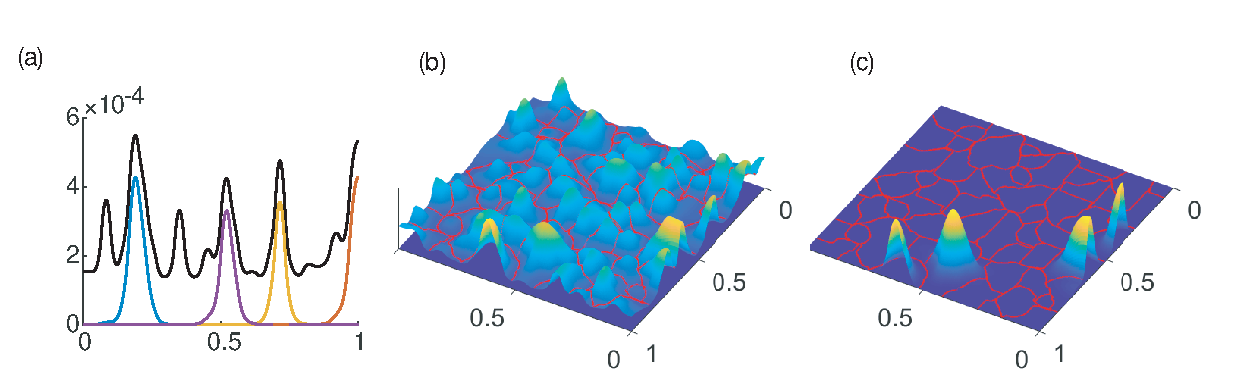
\includegraphics[width=\linewidth]{Fig1.eps}
\caption{(a) The landscape and first 4 eigenmodes obtained by simulating the system \eqref{anderson} and \eqref{landscape} with Neumann boundary condition. The black line represents the landscape and the colored lines represent the eigenmodes. (b) The landscape and corresponding valley lines in a two-dimensional case. Red lines represent the valley lines. (c) The first 4 eigenmodes and corresponding valley lines.}
\label{fig1}
\end{figure}

%Most works focus on Dirichlet boundary condition, but we would indicate that eigenmodes and eigenvalues may perform differently under different boundary conditions. As shown in Figure \ref{fig:4}, under Dirichlet and Neumann BC, difference of eigenmode is obvious, but egienvalues not. For larger eigenvalues, difference of eigenmodes are much larger.
%
%Figure shows the 2-d case. It's intersting that both eigenvalues and eigenmodes are totally different in 2-d case. 
%
%Eigenvalues under different boundary conditions performs differently in 1-d and 2-d case. Figure  shows the difference in respect of increasing rates.
%
%boundary condition is important in model, our work make sense.

\section{Limit behavior}\label{limit}

In this section, we focus on the limit behavior of the eigenmodes when the degree of randomness $K$ is very large. For simplicity, we assume that the potential function $V$ restricted to each sub-hypercube has the Bernoulli distribution \eqref{bernoulli}, which can only take the value of $0$ or $1$. Let
\begin{equation*}
D = \{x \in \Omega: V(x) = 0\}
\end{equation*}
denote the collection of sub-hypercubes at which the potential vanishes. We first consider the behavior of eigenmodes outside $D$. Let $x$ be the initial value of the reflecting diffusion $X_t$ solving the Skorokhod equation \eqref{reflecting}. When $x \notin D$, we have $V(X_s) = 1$ when $s$ is small, which implies that
\begin{equation*}
\int_{0}^{t} V(X_s) ds > 0, \quad \forall \; t > 0.
\end{equation*}
It thus follows from the probabilistic representation \eqref{probeigen} and the dominated convergence theorem that
\begin{equation}\label{largeK}
\lim_{K \rightarrow \infty} u(x) = 0, \quad \forall \; x \notin D.
\end{equation}
This shows that all eigenmodes must vanish outside $D$ in the limit of $K \rightarrow \infty$. In other words, when the the degree of randomness $K$ is very large, the eigenmodes can only localize in the subdomain at which the potential attains its minimum.

We next focus on the behavior of eigenmodes inside $D$. Clearly, $D$ can be decomposed as the disjoint union of several connected components:
\begin{equation*}
D = D_1 \cup D_2 \cup \cdots \cup D_N.
\end{equation*}
In the limit of $K\rightarrow\infty$, the eigenmode $u$ must satisfy the following local eigenvalue problem in each subdomain $D_k$:
\begin{equation}\label{subdomain}
\left\{
\begin{split}
& - L u = \lambda u \quad \textrm{in}\;\;\Omega, \\
& \quad g \frac{\partial u}{\partial n} + h u = 0 \quad \textrm{on}\;\;\partial D_k \cap \partial \Omega, \\
& \quad u = 0 \quad \textrm{on}\;\;\partial D_k \setminus \partial \Omega.
\end{split}
\right.
\end{equation}
Therefore, in the limit of $K \rightarrow \infty$, the spectrum of the Hamiltonian $H = - L + K V$ is composed of the local eigenvalues of the operator $-L$ in each subdomain $D_k$. If an eigenvalue of $H$ coincides with one of the local eigenvalues of $-L$ in $D_k$, then the corresponding eigenmode will be localized in $D_k$; conversely, if an eigenvalue of $H$ coincides with neither one of the local eigenvalues of $-L$ in $D_k$, then the corresponding eigenmode will not be localized in $D_k$. Based on the above discussion, if multiple subdomains $D_{k_1}, \cdots, D_{k_r}$ share a common local eigenvalue, then the corresponding eigenmode will have multiple peaks and the system will display \emph{multimodality}. In this case, the eigenmode is composed of the local eigenmodes of subdomains sharing a common eigenvalue.

Fig. \ref{fig2} (a) shows the potential, landscape and eigenmodes of a one-dimensional problem. We choose the parameter $K = 10^4$. Subdomains on which $V = 1$ is colored gray. One can see that the peaks of landscape and eigenmodes only appears on the subdomains where $V = 0$. Fig. \ref{fig2} (b) shows the potential and valley line of a two-dimensional problem. We choose the parameter $K = 10^4$. One can see that the connected components $D_1, \cdots, D_k$ are separated by the valley lines. That is, for a sufficient large $K$, subdomains divided by valley lines are consistent with the connected components of $D$.

\begin{figure}
\centering
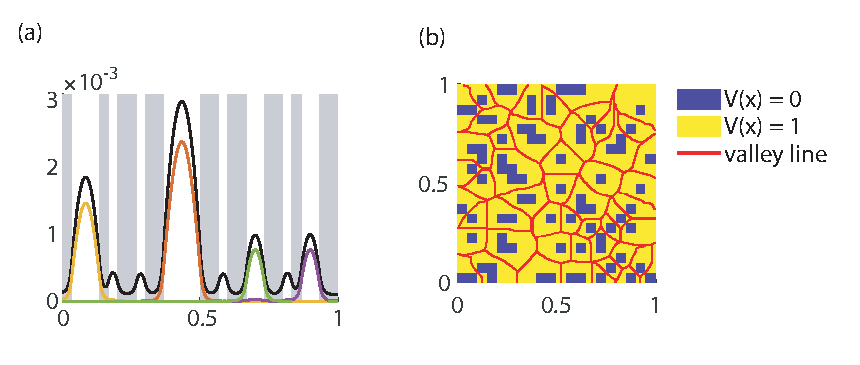
\includegraphics[width=\linewidth]{Fig2.eps}
\caption{(a) The potential, landscape and first 4 eigenmodes of a one-dimensional problem with Neumann boundary condition. The gray back ground represents that $V$ on the subdomian is $1$ and the white background represents $0$. The black line represents the landscape and the colored lines represent the eigenmodes. (b) The potential and valley lines in a two-dimensional problem with Neumann boundary condition. The yellow parts represent that $V$ on the subdomians are $1$ and the blue parts represent $0$. Red lines represent the valley lines.}
\label{fig2}
\end{figure}

\section{Probility of localization to the boundary}\label{prob}

\textbf{\color{red} The following discussion applies only to problem \eqref{anderson}}

\subsection{Localization to the boundary}

As shown in Fig \ref{fig1}, eigenmodes of a problem with Neumann or Robin boundary condition may localize to the boundary, only half of the peak appears in the domain. That is to say, the boundary value of some eigenmodes may be very large, even the maximum value on the whole domain may appear on the boundary. In this section, we will discuss the probability of localization to the boundary. For simplicity, we only consider the first eigenmode.

In one-dimensional problems, for a certain eigenmode, the probability of its localization to the boundary is defined as
\begin{equation}
P_b = \frac{\max\{|u(0)|, |u(1)|\}}{\max_{x \in \Omega} |u(x)|},
\end{equation}
and for two-dimensional problems, we can define the probability of localization to the edge as
\begin{equation}
P_e = \frac{\max_{x \in \partial\Omega} |u(x)|}{\max_{x \in \Omega} |u(x)|},
\end{equation}
and the probability of localization to the corner as
\begin{equation}
P_c = \frac{\max\{|u(0,0)|, |u(0,1)|, |u(1,1)|, |u(1,0)|\}}{\max_{x \in \Omega} |u(x)|}.
\end{equation}

When the boundary condition of the problem is Dirichlet, $P_b$, $P_e$ and $P_c$ are constantly $0$, and for Rboin and Neumann boundary condition, since the potential $V$ is randomly sampled from the Bernoulli distribution, $P_b$, $P_e$ and $P_c$ are random varaibles. Under such conditions, the probability of localization to the boundary, edge and corner under certain parameters are defined as the expectation of $P_b$, $P_e$ and $P_c$ respectively.

\subsection{Extended subdomains}

As shown in Section \ref{limit}, for large $K$, eigenmodes on the subdomain $D$ can be approximately regarded as the solution of the local eigenvalue problem \eqref{subdomain}. Further more, the first eigenmode of problem \eqref{anderson} must localize to the subdomain on which the eigenvalue of problem \eqref{subdomain} is the smallest. In one-dimensional problems, for Dirhclet boundary condition, the first eigenmode will localize to the longest subdomain. For Neumann boundary condition, we can transform it into Dirichlet boundary with the help of some symmetric properties.

For details, consider a Laplacian eigenvalue problem on an interval $D$ with left Neumann boundary condition and right Dirichlet boundary condition. Interval $D^{(e)}$ is twice as long as $D$. Laplacian eigenvalue problem on $D^{(e)}$ has both side Dirichlet boundary condition. It's easy to prove that the smallest eigenvalue on $D$ is equal to the smallest eigenvalue on $D^{(e)}$. What's more, the first eigenmode on $D^{(e)}$ can be obtained by the first eigenmode on $D$ through mirror symmetry. We call the $D^{(e)}$ \emph{extended subdomain}. Fig. \ref{fig3} (a) shows the first eigenmode on $D$ and $D^{(e)}$.

Precisely, extended subdomains can be defined as follows. For Neumann boundary conditions, the extended subdomain $D^{(e)}$ is equal to $D$ when $D \cup \partial \Omega = \phi$, and $D^{(e)}$ is twice as long as $D$ when $D \cup \partial \Omega \neq \phi$. According to the discussions in Section \ref{limit}, in one-dimensional problems, the first eigenmode of problem \eqref{anderson} will localize to the longest extended subdomain. In two-dimensional problems, we can define the extended subdomain similliary, in particular, the sub area near the corner will be extended twice. The conclusion turns to that the first eigenmode of problem \eqref{anderson} will localize to the extended subdomain on which Dirichlet eigenvalue is the smallest.

Fig. \ref{fig3} (b) and (c) shows the extended subdomains in one-dimensional and two-dimensional case respectively. Extended subdomains are surrounded by red lines. From the figure we can see, for a certain potential, subdomains are almost the same size, then the extended subdomains on the boundary has larger size and better symmetry, which cause the eigenmodes of problems with Neumann boundary condition are more likely to localize to the boundary.

\begin{figure}
\centering
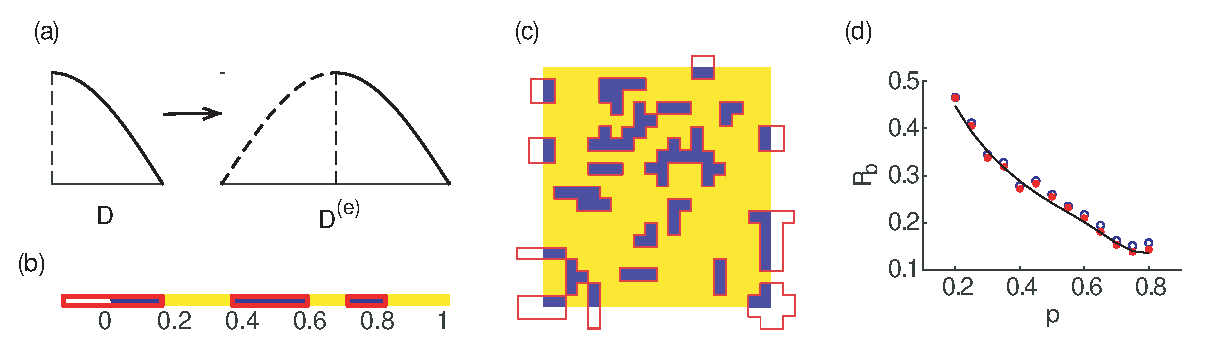
\includegraphics[width=\linewidth]{Fig3.eps}
\caption{(a) The first eigenmode of the problem on $D$ and $D^{(e)}$. (b) and (c) The extended subdomains in one-dimensional and two-dimensional case respectively. Blue parts are subdomians on which $V = 0$ and yellow parts represents $V = 1$. Subdomains $D$ are the blue parts and extended subdomains $D^{(e)}$ are surrounded by red lines. (d) Simulation results and theoretical predictions of the problility of localization to the boundary. Blue circles represents the simulation result of $P_b$, red stars represents the frequency of the event "the longest extended subdomain locates on the boundary" in the simulation, black line represents the thoretical prediction of $P_b$ from equation \eqref{bdprob}.}
\label{fig3}
\end{figure}

\subsection{A theoretical result for one-dimensional problems}

In one-dimensional problems, the whole domain $[0, 1]$ is divided uniformly into $N$ intervals. In each interval, the potential $V$ is constant with its value being sampled from the Bernoulli distribution. The values of the potential on different intervals are independent.

Suppose that the previous two intervals on which $V$ takes the value $1$ and $0$ respectively, let the number of following intervals on which $V$ takes the value $0$ to be a random variable $X$. $X$ takes the value $n$ means the values of $V$ on the next $n-1$ intervals are $0$ and the next $n$-th interval takes the value $1$. For a sufficient large $N$, $X$ approximately obeys the geometric distribution with parameter $p$.
$$ \mathbb{P}(X = n) = q^{n-1} p, $$
where $q = 1 - p$.

Similarly, the number of continuous intervals on which $V$ takes the value $1$ is a random variable $Y$ with distribution
$$ \mathbb{P}(Y = n) = p^{n-1} q. $$

In the whole interval, a subdomain on which $V = 0$ and $V = 1$ must appear alternately, which is called a \emph{period}. The average length of each period is $\Enum(X + Y) = \frac{1}{p q}$. So the average number of periods in the whole domain is $M = N p q$. In the average sense, we can approximately regard the whole domain consists of subintervals taking values $0$ and $1$ alternately with length $X_1, Y_1, \cdots, X_M, Y_M$. For a sufficient large $N$, random variables $X_1, Y_1, \cdots, X_M, Y_M$ are approximately independent.

For sufficient big $K$ and small $h$, the probability of "the first eigenmode localize to the boundary" is equal to the probability of the event that "the longest extended subdomain locates on the boundary". We can get its probability is
\begin{equation}\label{bdprob}
P_b = q^2 p^2 \sum_{k=1}^{\infty} q^{k-2} \sum_{n=1}^{k-1} (1 - q^{2 \max\{k-n,n\}-1})^{M-2} + p q^2 \sum_{n=1}^{\infty} (1 - p^{2 n-1})^{M-2} p^{n-1}.
\end{equation}
Detailed calculations are given in Appendix \ref{AppendixB1}.

Fig. \ref{fig3} (d) shows the simulation results and theoretical predictions. We choose parameters $K = 5 \times 10^4, h = 0.01$. The whole domain is divieded into $N = 50$ intervals. The theoretical prediction is in good agreement with the simulation. We randomly generate the potential $1000$ times to calucalte the mean value of the samples as the expectation of $P_b$.

\begin{remark}
Here we choose the parameter $h$ to be small but not $0$ to avoid multimodality, which will be discussed in section \ref{multimodality}. Under such conditions, if two extended subdomains have the same length, the first eigenmode will not localize to the boundary. This can help us avoid more complicated discussions.
\end{remark}

%\subsection{more simulation results}
%
%In following simulation, for one-dimensional problems, hole domain $[0,1]$ is divided into $50$ small intervals, for two-dimensional problems, $[0,1]^2$ is divided into $15 \times 15$ small squares. We randomly generate the potential $1000$ times to calucalte the mean value of the samples as the expectation of $P_b$, $P_e$ and $P_c$.
%
%\paragraph{relation of parameter h}
%
%The probability of localization to the boundary varies to $h$ with parameter $p=0.5, K=10^3$ is shown in the Fig. \ref{fig3} (e). In Robin boundary condition, when $h$ goes to infinity, the boundary approches Dirichlet, and when $h$ goes to $0$, the boundary approches Neumann.
%
%\paragraph{relation of parameter p}
%
%The probability of localization to the boundary varies to $p$ with parameter $h=1, K=10^3$ is shown in the Fig. \ref{fig3} (f). {\color{red} unfinished, how to explain this result?}
%
%\paragraph{relation of parameter K}
%
%The probability of localization to the boundary varies to $K$ with parameter $p=0.5, h=1$ is shown in the Fig. \ref{fig3} (g). {\color{red} unfinished, how to explain this result?}

\section{Multimodality}\label{multimodality}

As shown before, the first eigenmode will localize to the longest extended subdomain. When the longest two extended subdomains have the same length, both first and second eigenmodes will have two peaks and the first eigenvalue is approximately equal to the second. We call this \emph{multimodality}. Thus, the probability of multimodality is approximately equal to the probability of "the longest two extended subdomain are same in length". For higher dimensiional problems, results are similar. Multimodality appears when there exist two eigenvalues approximately equal.

Fig. \ref{fig4} (a) shows an example of multimodality. We choose the parameter $K = 10^4$ and the boundary condition is Neumann. The first and the second eigenvalue in the example are both $\lambda_1 = \lambda_2 = 681.5523$. In addation, one can not get information of multimodality from the landscape. Landscape can only tell us where eigenmodes might localize.

For Dirichlet boundary condition, we can get the probability of multimodality is
\begin{equation}\label{multiD}
P_D = 1 - p \sum_{n=1}^{\infty} (1 - p^{n-1})^{M-2} q^{n-1},
\end{equation}
and for Neumann boundary condition, probability of multimodality is
\begin{equation}\label{multiN}
\begin{split}
P_N = 1 - & q^2 (M-2) \sum_{n=1}^{\infty} (1 - q^{(n-1)/2})^2 (1 - q^{n-1})^{M-3} q^{n-1} p \\
- & 2 q^2 \sum_{n=1}^{\infty} (1 - q^{2n-1})^{M-2} (1 - q^{n-1}) q^{n-1} p \\
- & 2 p q (M-1) \sum_{n=1}^{\infty} (1 - q^{(n-1)/2}) (1 - q^{n-1})^{M-2} q^{n-1} p \\
- & 2 p q \sum_{n=1}^{\infty} (1 - q^{2n-1})^{M-1} q^{n-1} p \\
- & p^2 M \sum_{n=1}^{\infty} (1 - p^{n-1})^{M-1} q^{n-1} p.
\end{split}
\end{equation}
Detailed calculations are given in Appendix \ref{AppendixB2} and Appendix \ref{AppendixB3}.

Affected by calculation error, we can hardly observe that eigenvalues are exactly equal in practice, so we define that the multimodellity appears when the relative difference between the first and the second eigenvalue satisity $\frac{\lambda_2 - \lambda_1}{\lambda_1} < 0.02$.

Fig. \ref{fig4} (b) and (c) show the simulation results and theoretical predictions. We choose parameters $K = 3 \times 10^6$. The whole domain is divieded into $N = 50$ intervals. The theoretical prediction is in good agreement with the simulation.

\begin{figure}
\centering
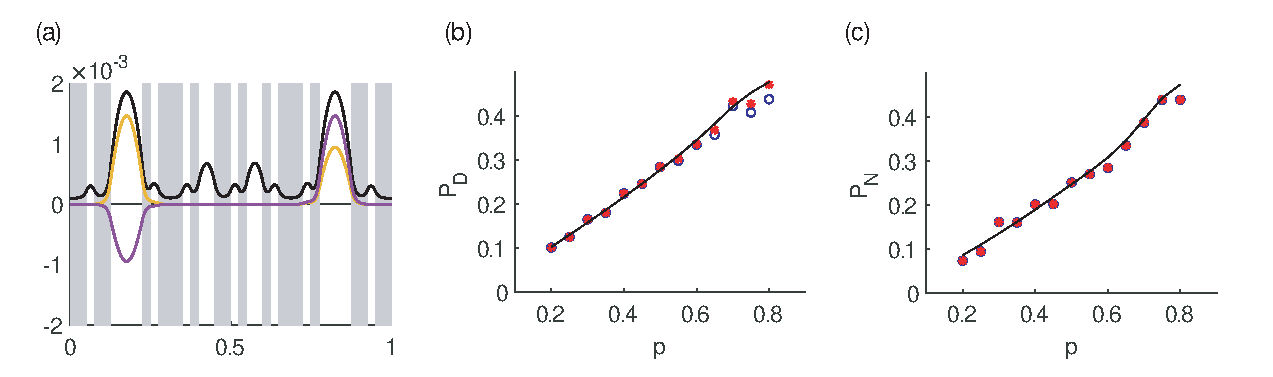
\includegraphics[width=\linewidth]{Fig4.eps}
\caption{(a) An example of multimodellity. The gray back ground represents that $V$ on the subdomian is $1$ and the white background represents $0$. The black line represents the landscape and the colored lines represent the eigenmodes. (b) and (c) Simulation results and theoretical predictions of the problility of multimodellity for Dirichlet and Neumann boundary condition respectively. Blue circles represents the frequency of multimodellity, red stars represents the frequency of the event "the longest two extended subdomain are same in length", black line represents the thoretical prediction obtained from equation \eqref{multiD} and \eqref{multiN}.}
\label{fig4}
\end{figure}

\section{Phase transition}\label{phase}

\subsection{Model of the phase transition}

Consider an one-dimensional problem with parabolic boundary condition. The potential $V$ is choosen as follows. As shown in Fig. \ref{fig5} (a), in the whole domain $[0,1]$, the values of $V$ are $0$ and $1$ alternately in these intervals with length $L_2/2, L_1, L_2, L_3, L_4, L_3, L_2/2$. The potential can be viewed as two wells $W_1$ and $W_2$ with length $L_1$ and $2 L_3$, while there is a barrier with length $L_4$ in the middle of the second well.

In the phase transion problem, $L_2$ should be big enough to seprate two wells and $L_4$ should be small. For detials, the parameters $L$ must satisify: $L_3 < L_1 < 2 L_3$ (two wells are approximately same in length), $L_4 < L_3 / 2$ (barrier should be short enough), $L_2 > L_1+ L_3 + L_4 + L_3$ ($L_2$ should be big enough to seperate the two wells), and total length $L_1 + 2 L_2 + 2L_3 + L_4 = 1$.

We choose $L_1 = 1/12, L_2 = 2/5, L_3= 1/20, L_4 = 1/60$. The first eigenmode and the second eigenmode for different $K$ is shown in Fig. \ref{fig5} (b). From the figure we can see, since the second well is longer, when $K$ is small, the barrier is not strong enough, so the first eigenmode will localize to $W_2$. When $K$ turns big, the first eigenmode will localize to $W_1$. With the increase of $K$, the left peak of the first eigenmode becomes higher and the right peak vanishes. Then location on which the first eigenmode localize will jump from $W_2$ to $W_1$, which is called \emph{phase transition}. The second eigenmode is the opposite of the first eigenmmode, location of the second eigenmode will jump from $W_1$ to $W_2$.

For details, we define the relative height of the left peak of eigenmode $u$ as 
\begin{equation}
F = \frac{\max_{x \in W_1} |u(x)|}{\max_{x \in W_1} |u(x)| + \max_{x \in W_2} |u(x)|}.
\end{equation}
It's obvious that in a certain range, the relative height $F$ of the first eigenmode increases with $K$. There exist a value of $K$ satisify the left peak and the right peak of the first eigenmode are equal in height ($F = 0.5$), which is defined as the \emph{critical point} $K_c$ in phase transition. The relative height $F$ will change rapidly when $K$ is near the critical point $K_c$.

\subsection{System decomposition}

In the phase transition problem, the potential has two wells. The two wells are so far apart that we can approximately assume that they have no influence on each other. So we can divide the problem into two subsystems, and discuss the eigenmode localize to $W_1$ and $W_2$ separately. As shown in Fig. \ref{fig5} (a), set the value of $V(x)$ in $W_1$ to $1$ and we can get $V_2(x)$. Similiarly, set the value in $W_2$ to $1$ and we can get $V_1(x)$. The original problem can be regarded as two subsystems $S_1$ and $S_2$ with potential $V_1(x)$ and $V_2(x)$ separately. For the first and the second eigenmode, the eigenmode localized to $W_1$ corresponds to subsystem $S_1$, and the other eigenmode corresponds to subsystem $S_2$. 

The paremeter $L$ is same as before, Fig. \ref{fig5} (c) shows the first and the second eigenmode of original system and the first eigenmode of two subsystems for $K = 800$. One can see that eigenmodes of subsystems are almost same with the eigenmodes of the original problem. Fig. \ref{fig5} (d) shows the eigenvalues of the original problem and subsystems for different $K$. The eigenvalues of subsystems are good approximation of the eigenvalues of the original problem.

Now we can give some detialed explaination of phase transion. Both the eigenvalues of $S_1$ and $S_2$ increase with the increasing of $K$, but they increase at different rates. When eigenvalue of $S_2$ is smaller, the right peak is dominant. As $K$ increasing, eigenvalue of subsystem two will exceed the other, then the minimum eigenvalue changes from one to the other. Then the localization of the peak will change from $W_2$ to $W_1$, the phase transition occurs. Similar to multimodality, phase transition occurs where the first and the second eigenvalues are equal.

\begin{figure}
\centering
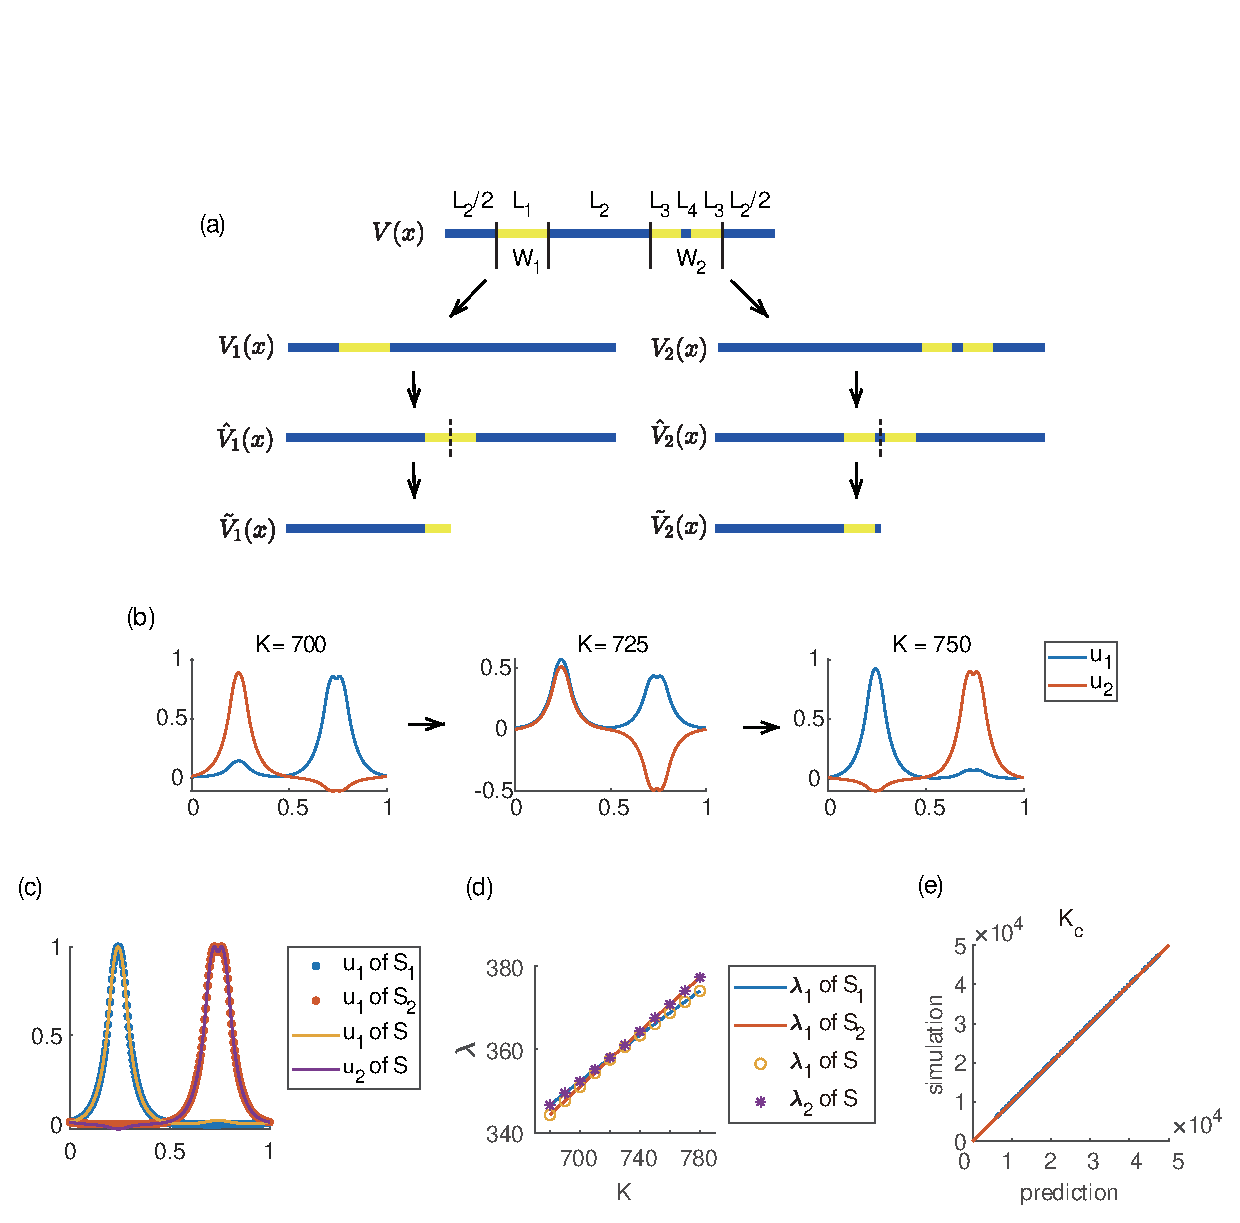
\includegraphics[width=\linewidth]{Fig5.eps}
\caption{(a) Potentials in phase transition problems. Blue parts are subdomians on which $V = 0$ and yellow parts represents $V = 1$. (b) The first eigenmode $u_1$ and the second eigenmode $u_2$ for different $K$. (c) and (d) Eigenmodes and eigenvalues of original system $S$ and two subsystems $S_1$ and $S_2$ respectively. (e) Simulation and prediction results on sample points. Each blue point represents a sample point whose x-axis reresents the prediction value of the critical point $K_c$ obtained by solving equation \eqref{phase0} and y-axis represents the simulation results. The red line is $x=y$, blue points are near the red line, which indicates that the predicted value is very close to the simulation result.}
\label{fig5}
\end{figure}

\subsection{Eigenvalue of the subsystems}

Consider the subsystem $S_1$, thanks to the periodicity, we can shift the potential freely. As shown in \ref{fig5} (a), we can move the well $W_1$ to the middle of interval without changing the eigenvalues. We can easily prove that eigenvalues of subsystem $S_1$ is equal to the eigenvalues of system with potential $\hat{V}_1$. The potential $\hat{V}_1$ is defined as
\begin{equation}
\hat{V}_1 = \left\{
\begin{split}
1 & \quad x \in [0, \frac{(1 - L_1)}{2}], \\
0 & \quad x \in [\frac{(1 - L_1)}{2}, \frac{(1 + L_1)}{2}], \\
1 & \quad x \in [\frac{(1 + L_1)}{2}, 1].
\end{split}
\right.
\end{equation}

Due to the symmetry, noting that the potential $\hat{V}_1$ satisifies $\hat{V}_1(x) = \hat{V}_1(1-x)$, then eigenmodes of the system also satisfy $u(x) = u(1-x)$. Because of the periodic boundary condition, we can prove that eigenmodes of subsystem satisfy $u'(0) = u'(1/2) = 0$. That is, eigenvalues of the system are equal to eigenvalues of problem on interval $[0, 1/2]$ with Neumann boundary condtion, whose potential $\tilde{V}_1$ is defined as
\begin{equation}
\tilde{V}_1(x) = \hat{V}_1(x) \qquad x \in [0, 1/2].
\end{equation}
Subsystem $S_2$ can be simplified similarly.

After simplified, for certain $K$, the first eigenvalue $\lambda$ of subsystem $S_1$ satisify the equation
\begin{equation}\label{phase1}
0 = D_1(K, \lambda) = \alpha \tan(\alpha x_0) - \beta \tanh(\beta (\frac12 - x_0)),
\end{equation}
where $\alpha = \sqrt{\lambda}, \beta = \sqrt{K - \lambda}, x_0 = L_1 / 2$.

Similarly, the first eigenvalue of subsystem $S_2$ satisify the equation
\begin{equation}\label{phase2}
\begin{split}
0 = D_2(K, \lambda) = & (\alpha^2 - \beta^2)(\mathrm{e}^{2 \beta x_2} + \mathrm{e}^{2 \beta (x_1+x_3)}) / (\mathrm{e}^{2 \beta (x_1+x_3)} - \mathrm{e}^{2 \beta x_2}) \\
+ & (\alpha^2 + \beta^2)(\mathrm{e}^{2 \beta x_3} + \mathrm{e}^{2 \beta (x_1+x_2)}) / (\mathrm{e}^{2 \beta (x_1+x_3)} - \mathrm{e}^{2 \beta x_2}) \\
+ & 2 \alpha \beta \cot(\alpha (x_1 - x_2))
\end{split},
\end{equation}
where $x_1 = L_4 / 2, x_2 = L_4 / 2 + L_3, x_3 = 1 / 2$. Detailed analysis are given in Appendix \ref{AppendixC}.

When pahse transition occurs, eigenvalue in both subsystem are equal, so the citical point $K_c$ and the ciritcal eigenvalue $\lambda_c$ satisify
\begin{equation}\label{phase0}
\left\{
\begin{split}
D_1(K_c, \lambda_c) = 0 \\
D_2(K_c, \lambda_c) = 0
\end{split}
\right.
\end{equation}

We generate $L_1, L_2, L_3, L_4$ randomly as our sample points. The sample points satisify $0.03 < L_3 < 0.055$, $1.3 L_3 < L_1 < 1.7 L_3$, $0.2 L_3 < L_4 < 0.4 L_3$ and $L_1 + 2 L_2 + 2 L_3 + L_4 = 1$. Fig. \ref{fig5} (e) shows the simulation and prediction results on these sample points. we can see  that the predicted value is very close to the simulation result. On these sample points, mean square error (MSE) of the citical point $K_c$ is $0.3947$, and MSE of the citical eigenvalue $\lambda_c$ is $9.1751$.

\begin{appendices}

\section{Proof of the Filochea-Mayboroda inequality}\label{AppendixA}

Let $(X, L)$ be the solution to the Skorokhod stochastic differential equation
\begin{equation*}
d X_t = b(X_t) dt + \sigma(X_t) d W_t + g(X_t) n(X_t) d L_t,
\end{equation*}
where $L$ is a continuous increasing process that increases when $X_t \in \partial \Omega$. For convenience, let
\begin{equation*}
Y_t = e^{\int_{0}^{t} h(X_s) d L_s - \int_{0}^{t} K V(X_s) ds}.
\end{equation*}
By Ito's formula, we have
\begin{equation*}
\begin{split}
du(X_t)Y_t =&\; u(X_t)Y_t[h(X_t)dL_t-KV(X_t)dt]
+\partial_iu(X_t)Y_tdX^i_t+\frac{1}{2}\partial_{ij}u(X_t)Y_t(dX^i_t)(dX^j_t)\\
=&\; u(X_t)Y_t[h(X_t)dL_t-KV(X_t)dt]+\partial_iu(X_t)b^i(X_t)Y_tdt
+\partial_iu(X_t)\sigma^i_j(X_t)Y_tdW^j_t\\
&\;+\partial_iu(X_t)g(X_t)n^i(X_t)Y_tdL_t+\frac{1}{2}\partial_{ij}u(X_t)a^{ij}(X_t)Y_tdt\\
=&\; \partial_iu(X_t)\sigma^i_j(X_t)Y_tdW^j_t+(Lu-KVu)(X_t)Y_tdt
+\left(g\frac{\partial u}{\partial n}+hu\right)(X_t)Y_tdL_t,
\end{split}
\end{equation*}
where we have used Einstein's summation convention: if the same index appears twice in any term, once as an upper index and once as a lower index, that term is understood to be summed over all possible values of that index. Since $L_t$ only increases when $X_t\in\partial\Omega$ and since $g\partial u/\partial n+hu = 0$ on $\partial\Omega$, we obtain
\begin{equation*}
du(X_t)Y_t = \partial_iu(X_t)\sigma^i_j(X_t)Y_tdW^j_t-\lambda u(X_t)Y_tdt.
\end{equation*}
This shows that
\begin{equation*}
u(X_t)Y_t = u(X_0)+\int_0^t\partial_iu(X_s)\sigma^i_j(X_s)Y_sdW^j_s-\lambda\int_0^tu(X_s)Y_sds.
\end{equation*}
Thus we have
\begin{equation*}
u(x) = \Enum_xu(X_t)Y_t+\lambda\Enum_x\int_0^t u(X_s)Y_sds.
\end{equation*}
Taking $t\rightarrow\infty$ in the above equation yields
\begin{equation*}
u(x) = \lambda\Enum_x\int_0^\infty u(X_s)Y_sds.
\end{equation*}
Recall that the localization landscape $w = w(x)$ is defined as the solution to the following PDE:
\begin{equation*}
\left\{
\begin{split}
& -Lw+KVw = 1 \quad \textrm{in}\;\;\Omega, \\
& \quad \frac{\partial w}{\partial n}+hw = 0 \quad \textrm{on} \; \; \partial \Omega,
\end{split}\right.
\end{equation*}
Similarly, the landscape has the following probabilistic representation:
\begin{equation*}
w(x) = \Enum_x\int_0^\infty Y_sds.
\end{equation*}

\section{Geometry distribution approximation}\label{AppendixB}

Let random variables $X_1, Y_1, \cdots, X_M, Y_M$ are independent, with distribution
$$ \mathbb{P}(X_k = n) = q^{n-1} p \quad \mathbb{P}(Y_k = n) = p^{n-1} q \qquad k = 1, 2, \cdots, M, $$
thus
$$ \mathbb{P}(X_k < n) = 1 - q^{n-1}, $$
where $q = 1 - p$ and $M = N p q$.

\subsection{Callculation of \eqref{bdprob}}\label{AppendixB1}

For Neumann boundary conditions, event "the longest extended subdoaim appears on the boundary" can be splitted into the following situations:

\paragraph*{situation 1}
$V(0) = V(1) = 0$ with probability $q^2$. Under such conditions, length of extended subdomains are $2 X_1, X_2, \cdots, X_{M-1}, 2 X_M$.

Then we have
\begin{equation*}
\begin{split}
  & \mathbb{P}(\text{the longest extended subdoaim appears on the boundary}) \\
= & \mathbb{P}(\max\{X_2, X_3, \cdots, X_{M-1}\} < 2 \max\{X_1, X_M\}) \\
= & \sum_{m,n=1}^{\infty} \mathbb{P}(\max\{X_2, X_3, \cdots, X_{M-1}\} < 2 \max\{m,  n\}) \mathbb{P}(X_1 = m) \mathbb{P}(X_M = n) \\
= & \sum_{m,n=1}^{\infty} [\mathbb{P}(X_k < 2 \max\{m,n\}) ]^{M-2} \mathbb{P}(X_1 = m) \mathbb{P}(X_M = n)\\
= & \sum_{m,n=1}^{\infty} (1 - q^{2 \max\{m,n\}-1})^{M-2} q^{m-1} p q^{n-1} p\\
= & \sum_{k=1}^{\infty} q^{k-2} p^2 \sum_{n=1}^{k-1} (1 - q^{2 \max\{k-n,n\}-1})^{M-2} 
\end{split}.
\end{equation*}

\paragraph*{situation 2}
$V(0) = 0, V(1) = 1$ with probability $p q$. Under such conditions, length of extended subdomains are $2 X_1, X_2, \cdots, X_M$.

Then we have
\begin{equation*}
\begin{split}
  & \mathbb{P}(\text{the longest extended subdoaim appears on the boundary}) \\
= & \mathbb{P}(\max\{X_2, X_3, \cdots, X_{M}\} < 2 X_1) \\
= & \sum_{n=1}^{\infty} \mathbb{P}(\max\{X_2, X_3, \cdots, X_{M-1}\} < 2 n) \mathbb{P}(X_1 = n) \\
= & \sum_{n=1}^{\infty} [\mathbb{P}(X_k < 2 n)]^{M-1} \mathbb{P}(X_1 = n)\\
= & q \sum_{n=1}^{\infty} (1 - p^{2 n-1})^{M-2} p^{n-1}
\end{split}.
\end{equation*}

\paragraph*{situation 3}
$V(0) = 1, V(1) = 0$ with probability $p q$. Under such conditions, length of extended subdomains are $2 X_1, X_2, \cdots, X_M$. It can be calculated simillary to situation 2.

In summary, probability of localize to the boundary is
\begin{equation*}
P_b = q^2 p^2 \sum_{k=1}^{\infty} q^{k-2} \sum_{n=1}^{k-1} (1 - q^{2 \max\{k-n,n\}-1})^{M-2} + p q^2 \sum_{n=1}^{\infty} (1 - p^{2 n-1})^{M-2} p^{n-1}.
\end{equation*}

\subsection{Calculation of \eqref{multiD}}\label{AppendixB2}

For Dirichlet Boundary, we have
\begin{equation*}
\begin{split}
P_D = & \mathbb{P}(\text{there is a unique longest subdomain}) \\
= & \sum_{k=1}^{M} \mathbb{P}(\max\{X_1, X_2, \cdots, X_{k-1}, X_{k+1}, \cdots, X_{M}\} < X_k) \\
= & M \; \mathbb{P}(\max\{X_{2}, X_{3}, \cdots, X_{M}\} < X_1) \\
= & M \sum_{n=1}^{\infty} \mathbb{P}(\max\{X_2, X_3, \cdots, X_{M-1}\} < n) \mathbb{P}(X_1 = n) \\
= & M \sum_{n=1}^{\infty} [\mathbb{P}(X_k < n)]^{M-1} \mathbb{P}(X_1 = n)\\
= & M \sum_{n=1}^{\infty} (1 - p^{n-1})^{M-1} q^{n-1} p
\end{split}.
\end{equation*}

\subsection{Calculation of \eqref{multiN}}\label{AppendixB3}

For Neumann Boundary, probability of "there is a unique longest extended subdomain" can be splitted into the following situations:

\paragraph*{situation 1}
$V(0) = V(1) = 0$ with probability $q^2$. We have
\begin{equation*}
\begin{split}
  & \mathbb{P}(\text{there is a unique longest subdomain}) \\
= & \sum_{k=2}^{M-1} \mathbb{P}(\max\{2 X_1, X_2, \cdots, X_{k-1}, X_{k+1}, \cdots, 2 X_{M}\} < X_k) \\
+ & \mathbb{P}(\max\{X_2, \cdots, X_{M-1}, 2 X_M\} < 2 X_1) \\
+ & \mathbb{P}(\max\{2 X_1, X_2, \cdots, X_{M-1}\} < 2 X_M) \\
= & (M-2) \mathbb{P}(\max\{2 X_1, X_3 \cdots, 2 X_{M}\} < X_2) \\
+ & 2 \mathbb{P}(\max\{X_2, \cdots, X_{M-1}, 2 X_M\} < 2 X_1) \\
= & (M-2) \sum_{n=1}^{\infty} \mathbb{P}(\max\{2 X_1, X_3 \cdots, 2 X_{M}\} < n) \mathbb{P}(X_2 = n) \\
+ & 2 \sum_{n=1}^{\infty} \mathbb{P}(\max\{X_2, \cdots, X_{M-1}, 2 X_M\} < 2 n) \mathbb{P}(X_1 = n) \\
= & (M-2) \sum_{n=1}^{\infty} [\mathbb{P}(2 X_k < n)]^2 [\mathbb{P}(X_k < n)]^{M-3} \mathbb{P}(X_2 = n) \\
+ & 2 \sum_{n=1}^{\infty} [\mathbb{P}(X_k < 2 n)]^{M-2} \mathbb{P}(X_k < n) \mathbb{P}(X_1 = n) \\
= & (M-2) \sum_{n=1}^{\infty} (1 - q^{(n-1)/2})^2 (1 - q^{n-1})^{M-3} q^{n-1} p \\
+ & 2 \sum_{n=1}^{\infty} (1 - q^{2n-1})^{M-2} (1 - q^{n-1}) q^{n-1} p
\end{split}.
\end{equation*}

\paragraph*{situation 2}
$V(0) = 0, V(1) = 1$ with probability $p q$. We have
\begin{equation*}
\begin{split}
  & \mathbb{P}(\text{there is a unique longest subdomain}) \\
= & \sum_{k=2}^{M} \mathbb{P}(\max\{2 X_1, X_2, \cdots, X_{k-1}, X_{k+1}, \cdots, X_{M}\} < X_k) \\
+ & \mathbb{P}(\max\{X_2, \cdots, X_{M-1}, X_M\} < 2 X_1) \\
= & (M-1) \mathbb{P}(\max\{2 X_1, X_3 \cdots, X_{M}\} < X_2) \\
+ & \mathbb{P}(\max\{X_2, \cdots, X_{M-1}, X_M\} < 2 X_1) \\
= & (M-1) \sum_{n=1}^{\infty} \mathbb{P}(\max\{2 X_1, X_3 \cdots, X_{M}\} < n) \mathbb{P}(X_2 = n) \\
+ & \sum_{n=1}^{\infty} \mathbb{P}(\max\{X_2, \cdots, X_{M-1}, X_M\} < 2 n) \mathbb{P}(X_1 = n) \\
= & (M-1) \sum_{n=1}^{\infty} \mathbb{P}(2 X_k < n) [\mathbb{P}(X_k < n)]^{M-2} \mathbb{P}(X_2 = n) \\
+ & \sum_{n=1}^{\infty} [\mathbb{P}(X_k < 2 n)]^{M-1} \mathbb{P}(X_1 = n) \\
= & (M-1) \sum_{n=1}^{\infty} (1 - q^{(n-1)/2}) (1 - q^{n-1})^{M-2} q^{n-1} p \\
+ & \sum_{n=1}^{\infty} (1 - q^{2n-1})^{M-1} q^{n-1} p
\end{split}.
\end{equation*}

\paragraph*{situation 3}
$V(0) = 1, V(1) = 0$ with probability $p q$. It can be calculated simillary to situation 2.

\paragraph*{situation 4}
$V(0) = 1, V(1) = 1$ with probability $p^2$. It can be calculated simillary to Dirichlet boundary condition.

In summary, probability of multimodellity on Neumann boundary condition is
\begin{equation*}
\begin{split}
P_N = 1 - & q^2 (M-1) \sum_{n=1}^{\infty} (1 - q^{(n-1)/2}) (1 - q^{n-1})^{M-2} q^{n-1} p \\
- & 2 q^2 \sum_{n=1}^{\infty} (1 - q^{2n-1})^{M-1} q^{n-1} p \\
- & 2 p q (M-1) \sum_{n=1}^{\infty} (1 - q^{(n-1)/2}) (1 - q^{n-1})^{M-2} q^{n-1} p \\
- & 2 p q \sum_{n=1}^{\infty} (1 - q^{2n-1})^{M-1} q^{n-1} p \\
- & p^2 M \sum_{n=1}^{\infty} (1 - p^{n-1})^{M-1} q^{n-1} p
\end{split}.
\end{equation*}

\section{Calculation of \eqref{phase1} and \eqref{phase2}}\label{AppendixC}

\subsection{subsystem on $W_1$}

Consider an one-dimensional eigenvalue problem with Neumann boundary condition in $[0, 1/2]$. In the interval $[0, x_0]$, $V$ takes the value $1$ and in $[x_0, 1/2]$ takes $0$, where $x_0 = L_1/2$.

We define $\alpha = \sqrt{\lambda}, \beta = \sqrt{K - \lambda}$. in the interval $[0, x_0]$, the eigenmode can be written as
\begin{equation*}
u(x) = A \sin(\alpha x) + B \cos(\alpha x) \qquad u'(x) = A \alpha \cos(\alpha x) - B \alpha \sin(\alpha x),
\end{equation*}
and in the interval $[x_0, 1/2]$,
\begin{equation*}
u(x) = C \exp(\beta x) + D \exp(-\beta x) \qquad u'(x) = C \beta \exp(\beta x) - D \beta \exp(-\beta x),
\end{equation*}
where $A ,B, C, D$ are the parameter to be determined.

According to the Neumann boundary condition and the continuity of the eigenmode, we have
\begin{equation*}
\begin{split}
u'(0) & = A \alpha = 0 \\
u'(1/2) & = C \beta \exp(\beta/2) - D \beta \exp(-\beta/2) = 0 \\
u(x_0) & = A \sin(\alpha x_0) + B \cos(\alpha x_0) = C \exp(\beta x_0) + D \exp(-\beta x_0) \\
u'(x_0) & = A \alpha \cos(\alpha x_0) - B \alpha \sin(\alpha x_0) = C \beta \exp(\beta x_0) - D \beta \exp(-\beta x_0)
\end{split},
\end{equation*}
that is
\begin{equation*}
\begin{split}
\left[\begin{array}{cccc} \alpha & 0 & 0 & 0\\ 0 & 0 & \beta \mathrm{e}^{\frac{\beta}{2}} & - \beta \mathrm{e}^{-\frac{\beta}{2}}\\ \sin\!\left(\alpha x_0\right) & \cos\!\left(\alpha x_0\right) & - \mathrm{e}^{\beta x_0} & - \mathrm{e}^{- \beta x_0}\\ \alpha \cos\!\left(\alpha x_0\right) & - \alpha \sin\!\left(\alpha x_0\right) & - \beta \mathrm{e}^{\beta x_0} & \beta \mathrm{e}^{- \beta x_0} \end{array}\right]
\left[\begin{array}{c} A \\ B \\ C \\ D \end{array}\right]
=
\left[\begin{array}{c} 0 \\ 0 \\ 0 \\ 0 \end{array}\right]
\end{split}.
\end{equation*}

The existence of solutions is equivalent to
\begin{equation*}
\det(A) = \alpha \mathrm{e}^{2 \beta x_0} \sin\!\left(\alpha x_0\right) - \beta \mathrm{e}^{\beta} \cos\!\left(\alpha x_0\right) + \alpha \mathrm{e}^{\beta} \sin\!\left(\alpha x_0\right) + \beta \mathrm{e}^{2 \beta x_0} \cos\!\left(\alpha x_0\right) = 0,
\end{equation*}
that is
\begin{equation*}
D_1(K, \lambda) = \alpha \tan(\alpha x_0) - \beta \tanh(\beta (\frac12 - x_0)) = 0.
\end{equation*}

\subsection{subsystem on $W_2$}

Consider the an one-dimensional eigenvalue problem with Neumann boundary condition in $[0, 1/2]$. In the interval $[0, x_1]$ and $[x_2, 1/2]$, $V$ takes the value $1$ and in $[x_1, x_2]$, $V$ takes $0$, where $x_1 = L_4/2, x_2 = L_4/2 + L_3$.

In the interval $[0, x_1]$, the eigenmode can be written as
\begin{equation*}
u(x) = A \exp(\beta x) + B \exp(-\beta x) \qquad u'(x) = A \beta \exp(\beta x) - B \beta \exp(-\beta x),
\end{equation*}
and in the interval $[x_1, x_2]$,
\begin{equation*}
u(x) = C \sin(\alpha x) + D \cos(\alpha x) \qquad u'(x) = C \alpha \cos(\alpha x) - D \alpha \sin(\alpha x),
\end{equation*}
and in the interval $[x_2, 1/2]$,
\begin{equation*}
u(x) = E \exp(\beta x) + F \exp(-\beta x) \qquad u'(x) = E \beta \exp(\beta x) - F \beta \exp(-\beta x),
\end{equation*}
where $A ,B, C, D, E, F$ are the parameter to be determined.

According to the Neumann boundary condition and the continuity of the eigenmode, we have
\begin{equation*}
\begin{split}
u'(0) & = A \beta - B \beta = 0 \\
u(x_1) & = A \exp(\beta x_1) + B \exp(-\beta x_1) = C \sin(\alpha x_1) + D \cos(\alpha x_1) \\
u'(x_1) & = A \beta \exp(\beta x_1) - B \beta \exp(-\beta x_1) = C \alpha \cos(\alpha x_1) - D \alpha \sin(\alpha x_1) \\
u(x_2) & = C \sin(\alpha x_2) + D \cos(\alpha x_2) = E \exp(\beta x_2) + F \exp(-\beta x_2) \\
u'(x_2) & = C \alpha \cos(\alpha x_2) - D \alpha \sin(\alpha x_2) = E \beta \exp(\beta x_2) - F \beta \exp(-\beta x_2) \\
u'(1/2) & = E \beta \exp(\beta/2) - F \beta \exp(-\beta/2) = 0
\end{split},
\end{equation*}
that is
\begin{equation*}
\begin{split}
\left[\begin{array}{cccccc} 1 & -1 & 0 & 0 & 0 & 0\\ \mathrm{e}^{\beta x_1} & \mathrm{e}^{- \beta x_1} & - \sin\!\left(\alpha x_1\right) & - \cos\!\left(\alpha x_1\right) & 0 & 0\\ \beta \mathrm{e}^{\beta x_1} & - \beta \mathrm{e}^{- \beta x_1} & - \alpha \cos\!\left(\alpha x_1\right) & \alpha \sin\!\left(\alpha x_1\right) & 0 & 0\\ 0 & 0 & \sin\!\left(\alpha x_2\right) & \cos\!\left(\alpha x_2\right) & - \mathrm{e}^{\beta x_2} & - \mathrm{e}^{- \beta x_2}\\ 0 & 0 & \alpha \cos\!\left(\alpha x_2\right) & - \alpha \sin\!\left(\alpha x_2\right) & - \beta \mathrm{e}^{\beta x_2} & \beta \mathrm{e}^{- \beta x_2}\\ 0 & 0 & 0 & 0 & \mathrm{e}^{\frac{\beta}{2}} & - \mathrm{e}^{-\frac{\beta}{2}} \end{array}\right]
\end{split}.
\end{equation*}

The existence of solutions is equivalent to
\begin{equation*}
\begin{split}
& \alpha^2 \mathrm{e}^{2 \beta (x_{1} + x_{2})}  + \alpha^2 \mathrm{e}^{2 \beta (x_{1} + x_{3})} \\
+ & \beta^2 \mathrm{e}^{2 \beta (x_{1} + x_{2})} - \beta^2 \mathrm{e}^{2 \beta (x_{1} + x_{3})} \\
+ & \alpha^2 \mathrm{e}^{2 \beta x_{2}}  + \alpha^2 \mathrm{e}^{2 \beta x_{3}} \\
- & \beta^2 \mathrm{e}^{2 \beta x_{2}} + \beta^2 \mathrm{e}^{2 \beta x_{3}} \\
+ & 2 \alpha \beta \mathrm{e}^{2 \beta (x_{1} + x_{3})} \cot(\alpha (x_{1} - x_{2})) - 2 \alpha \beta \mathrm{e}^{2 \beta x_{2}} \cot(\alpha (x_{1} - x_{2})) = 0
\end{split},
\end{equation*}
that is
\begin{equation*}
\begin{split}
0 = D_2(K, \lambda) = & (\alpha^2 - \beta^2)(\mathrm{e}^{2 \beta x_2} + \mathrm{e}^{2 \beta (x_1+x_3)}) / (\mathrm{e}^{2 \beta (x_1+x_3)} - \mathrm{e}^{2 \beta x_2}) \\
+ & (\alpha^2 + \beta^2)(\mathrm{e}^{2 \beta x_3} + \mathrm{e}^{2 \beta (x_1+x_2)}) / (\mathrm{e}^{2 \beta (x_1+x_3)} - \mathrm{e}^{2 \beta x_2}) \\
+ & 2 \alpha \beta \cot(\alpha (x_1 - x_2))
\end{split},
\end{equation*}
where $x_3 = \frac12$.

\end{appendices}

\section*{Acknowledgements}
The authors acknowledge support from the NSAF grant in National Natural Science Foundation of China (NSFC) with grant No. U1930402.

\setlength{\bibsep}{5pt}
\small\bibliographystyle{nature}
\bibliography{localization}

\end{document}
